\section{Transaktionen}
Transaktionsabbrüche durch Integritätsverletzungen, Konsistenzbedinungen,\\ Speicher voll, Verbindungsabbruch, Systemausfall ...

\subsection{Anomalien vs isolation level}
\halfpage{\begin{enumerate}
\item Lost-Update: Überschriebene Änderungen bei parallelen Transaktionen\\
isolation level: read uncommitted
\item Dirty-Read: Lesen eines nicht committeten Wertes\\
isolation level: read committed
\item Unrepeatable Read: identische abfragen mit verschiedene Ergebnisse durch commit zweiter Transaktion\\
isolation level: repeatable read
\item Phantom Read: Einfügen von Datensätzen durch andere Transaktion \\
isolation level: serializable
\item ---\\isolation level: Snapshots (Multi-Version-Concurrency-Control) keine Lesesperren, änderungen erzeugen kopie

\end{enumerate}}\\

\textbf{Serialisierbar:} Gleiches Ergebnis wie bei hintereinanderausführung der Transaktion



z.B. $R_1(a), \textcolor{red}{W_2(a)}, R_3(a), \textcolor{green}{W_1(a)}$

\begin{minipage}{0.06\textwidth}
\tikzset{ LabelStyle/.style = { rectangle, rounded corners, draw, minimum width = 2em, font =fseries }, VertexStyle/.append style = { inner sep=5pt, font = \Large\bfseries}, EdgeStyle/.append style = {->,bend left =20}}
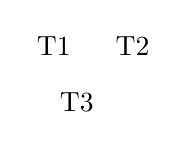
\begin{tikzpicture}
\tikzset{EdgeStyle/.append style = {->,bend left =20,red}}
\node(1){T1}; \node(2)[right of=1]{T2}; \node(3)[below left of=2]{T3};

\Edge(1)(2){a}; \Edge(2)(3){a}; 
\tikzset{EdgeStyle/.append style = {green}}
\Edge(2)(1){a}; \Edge(3)(1){a}; 
\end{tikzpicture}
\end{minipage}
=> Zyklus => nicht serialisierbar



\subsection{Zwei-Phasen-Protokoll:} Sperren werden erst am Transaktionsende (vor commit) wieder freigegeben

Sperren: Shared-Locks (s) beim Lesen, Exklusiv-Locks (X) beim Schreiben
$R_1(a),R_2(a),W_1(a),W_2(a)$

\begin{tabular}{|c|c|}
\hline
T1 & T2 \\
\hline
Slock(a), read(a); & \\
& Slock(a), read(a);\\
Wait(Xlock(a)) & \\
& Wait(Xlock(a))\\
& DEADLOCK => Rollback;\\
write(a)&\\
unlock(a);&\\
commit;&\\
\hline
\end{tabular}\\ \\ \\



\section{Anfrageverarbeitung}

SQL -> Query Execution Plan:\\
Parsen der Anfrage -> Operatorengraph; // hierbei Standardisieren und vereinfachen  \\
\textbf{KNF} : (a and b) or (c and d); \\
\rule{2em}{0em}deMorgan: $\overline{a AND b} = \overline{a} OR \overline{b}$\\
\rule{2em}{0em}\textcolor{white}{deMorgan :} $\overline{a OR b} = \overline{a} AND \overline{b}$

\definecolor{darkgreen}{rgb}{0.2,0.8,0.2}
\newcommand{\proj}{\textcolor{red}{\ensuremath{\pi_{k.nr,p.nr}}}}
\newcommand{\joink}{\textcolor{darkgreen}{\ensuremath{\bowtie_{k.knr = a.knr}}}}
\newcommand{\joina}{\textcolor{darkgreen}{\ensuremath{\bowtie_{a.anr = p.anr}}}}
\newcommand{\selk}{\textcolor{blue}{\ensuremath{\sigma_{k.name = 'x'}} }}
\newcommand{\selor}{\textcolor{blue}{\ensuremath{\sigma_{a.anr > 10~OR~k.knr >10 }}}}
\newcommand{\grpi}[1]{\textcolor{gray}{ \ensuremath{\pi_{ #1 }} }}
\newcommand{\colobr}[3]{\textcolor{#1}{$\underbrace{\textcolor{black}{#2}}_{#3}$}}

\begin{minipage}{0.25\textwidth}
\textbf{\textcolor{red}{HINWEIS:}}von unten nach oben konstruieren.\\\\
SELECT \colobr{red}{k.name, p.nr}{ \proj } \\
FROM Knd k JOIN Auftr a \colobr{darkgreen}{ ON k.knr = a.knr}{\joink} \\
JOIN Auftrpos p \colobr{darkgreen}{ ON a.anr =p.anr}{\joina} \\
WHERE \colobr{blue}{k.name = 'x'}{\selk} AND\\
\rule{2em}{0em}\colobr{blue}{(a.anr > 10 OR k.knr >10)}{\selor}
\end{minipage}
\begin{minipage}{0.25\textwidth}
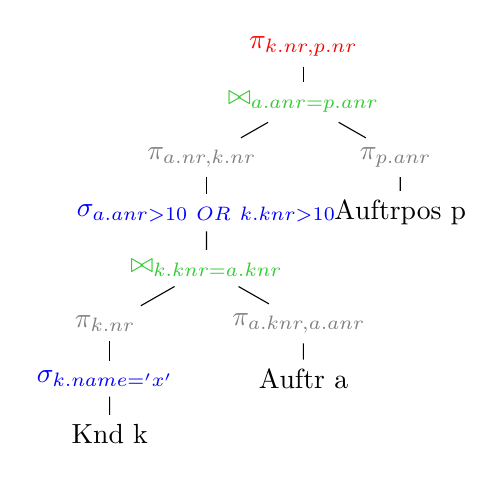
\begin{tikzpicture}[level distance=2em,sibling distance=5.5em ,level 2/.style={sibling distance=7em} ]
\node{\proj} 
child{ node{\joina}
child{ node{\grpi{a.nr,k.nr}}
child{ node{\selor}
child{ node{\joink}
child{ node{\grpi{k.nr}}
child{ node{\selk}
child{ node{Knd k}}}}
child{ node{\grpi{a.knr,a.anr}}
child{ node{Auftr a}}}
}}}
child{ node{\grpi{p.anr}}
child{ node{Auftrpos p}
}}}
;
\end{tikzpicture}
\end{minipage}



\subsection{Kostenschätzung}
Anhand von Statistiken, Histogrammen, etc.; evtl. Hints für Optimizer

\textbf{Kardinalität}: |a|: Anzahl der gelieferten Datensätze \\
\textbf{Selektivität}: 
Sel(a) = $\dfrac{zur"uckgegebene DS}{gesamt DS}$\\
NumBlocks: $\dfrac{|R|\cdot Gr"osse_{Datensatz}}{Blocksize}$

Levels(I(R,A)): Höhe des Index auf A


Attribut = 'sth' => Sel(A) = $\dfrac{1}{|A|}$

Attribut IN $\{c_1,c_2, \dots , c_n\}$ => Sel(A) = n / |A|

A >c => Sel(A) = $\dfrac{A_{max} -c }{A_{max} - A_{min}}$

$P_1~AND~P_2$ => $Sel(P_1) \cdot Sel(P_2)$

$P_1~OR~P_2$ => $Sel(P_1) + Sel(P_2) + Sel(P_1~AND~P_2)$



\section{Fehlerbehandlung}
\textbf{Lokaler Fehler} (in Transaktion): Rollback der Transaktion

\textbf{Verlust des internen Speichers:} Abarbeiten des Logs.\\
1. Redo-lauf (durchführen der geloggten änderungen); \\
2. Undo-lauf: rollback nicht committeter änderungen;

\textbf{Verlust des externen Speichers:} Backup einspielen, inkrementell log-einspielen


\textbf{Write-Ahead-Logging:} logging vor commit, bei rollback wiederherstellen aus log;\\
Log beinhaltet Undo- und Redo-Informationen; (vor und nach zustand)\\
\textit{logisches Logging:} protokollierung der ausgeführten Befehle\\
\textit{physisches Logging:} Kopien der Datensätze (vor/nach)

\textbf{Steal-noforce:}
Steal: gepufferte, uncommittete seiten können von anderer Transaktion eingelagert werden, zusammen mit zugehörigem Undo-logeintrag\\
NoForce: committete Seiten werden sofort im Redo-log vermerkt, irgendwann auf Platte geschrieben



\textbf{Recovery time objective:} max. ausfallzeit; \textbf{recovery point objective:} max. Datenverlust

\section{Dateiorganisation}
\textbf{Heap} Speichern von Datensätzen in Einfügereihenfolge => unsortiert\\
Einfügen am ende, löschen suchen und setzen eines Löschbits;

\textbf{Sequentielle}: sortierte speicherung;\\
einfügen: suchen, einfügen und Seite sortieren; löschen: suchen und löschbit setzen;

\textbf{Index:} B-Baum-Struktur; \\ 
\textbf{clustered Index:} Segmente selbst sind sortiert ( vgl. Sequentiell)  


\section{Plan-Operatoren}
\halfpage{\begin{itemize}
\item \textbf{Full-Table-Scan:} durchsuche gesamte Tabelle: Cost = NumBlocks(R)
\item \textbf{Index-Scan:} Suche anhand index: Cost = Levels(Index) + Sel(P) $\cdot$|R|
\item \textbf{Nested-Loop-Join:} für jeden Block: durchlaufe die andere Tabelle\\
Ohne Index: Cost= NumBlocks(R) * NumBlocks(S) ; \\
mit Index Cost= NumBlocks(R) * Cost(IndexScan)
\item \textbf{Merge-Join:} Sortiere die Relationen nach Join-Attribut; \\paralleles Durchlaufen der Paare in den sortierten Relationen;\\
Cost: Cost(Sort(R)) +Cost(Sort(S)) + NumBlocks(S) + NumBlocks(R)
\item \textbf{Hash-Join:} Teile kleinere Relation K in h Abschnitte, wird im RAM gehalten;\\
durchlaufe die Abschnitte: Erstelle Hashtabelle, prüfe für jeden Datensatz der 2. Relation JOIN-Bedingung mit den Zugehörigen Werten; Cost: NumBlocks(R) + x * NumBlocks(S)

\end{itemize}}